\documentclass{beamer}
\usepackage{amsthm}
\usepackage{amsmath,amssymb}
\usepackage{graphicx}

\newtheorem*{conj}{Conjecture}
\newtheorem*{prop}{Proposition}
\newtheorem*{defin}{Definition}

\title{Week 2 Presentation}
\author{Max Comstock}
\date{Summer 2014}

\begin{document}

\frame{\titlepage}

\begin{frame}
\frametitle{Sheehan's Conjecture (1975)}
\begin{conj}
  Every 4-regular graph has at least two Hamiltonian cycles.
\end{conj}
\end{frame}

\begin{frame}
\frametitle{A way to algebraically encode Hamiltonian cycles}
\begin{prop}
  Let $G = (V,A)$ be a simple directed graph on vertices $V = \{1, \ldots, n\}$. Assume that the characteristic of $\mathbb{K}$ is relatively prime to $n$ and that $z \in \mathbb{K}$ is a primitive $n$-th root of unity. Consider the following system in $\mathbb{K}[x_1, \ldots, x_n]$:
  \begin{align*}
    H_G = \{x_i^n - 1 = 0, \prod_{j \in \delta^+(i)} (z x_i - x_j) = 0 \, : \, i \in V\}
  \end{align*}
  Here, $\delta^+(i)$ denotes those vertices $j$ which are connected to $i$ by the arc going from $i$ to $j$ in $G$. The system $H$ has a solution over $\mathbb{K}$ if and only if $G$ has a Hamiltonian cycle.
\end{prop}
Source: ``Recognizing Graph Theoretic Properties with Polynomial Ideals'' by J.A. De Loera, C. Hillar, P.N. Malkin, and M. Omar.
\end{frame}

\begin{frame}
\frametitle{Simple case: directed graphs}
\begin{defin}
  Let $z$ be a fixed primitive $k$-th root of unity. If $C$ is a directed cycle of length $k$ in a directed graph, with vertex set $\{v_1, \ldots, v_k\}$, the cycle encoding of $C$ is the following set of $k$ polynomials:
  \begin{align*}
    g_i = \left \{ \begin{matrix} x_{v_{k-i}} - z^{k-i} x_{v_k} & i = 1, \ldots, k-1\\ x_{v_k}^k - 1 & i = k \end{matrix} \right ..
  \end{align*}
\end{defin}
Note: define $H_{G,C} = \langle g_1,\ldots, g_i \rangle$. The $g_i$'s form a reduced Gr\"obner basis (which must be unique) for $H_{G,C}$.
\end{frame}

\begin{frame}
\frametitle{Simple example}
\begin{center}
  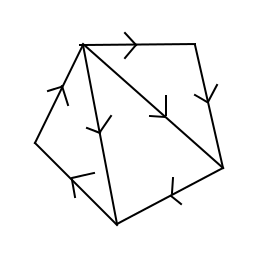
\includegraphics[width=1in]{pent2.png}
\end{center}
Let $z$ be a primitive 5\textsuperscript{th} root of unity. We are looking for solutions to the system $H$:
\begin{align*}
  x_i^5 - 1 &= 0 \quad 1 \leq i \leq 5\\
  (z x_1 - x_2) (z x_1 - x_3) (z x_1 - x_4) &= 0\\
  z x_2 - x_3 &= 0\\
  z x_3 - x_4 &= 0\\
  z x_4 - x_5 &= 0\\
  z x_5 - x_1 &= 0
\end{align*}
\end{frame}

\begin{frame}
\frametitle{Simple example (continued)}
Process for a single Hamiltonian cycle: Let $H_G$ be the ideal generated by the polynomials in the system $H$. If we find a Gr\"obner basis for $H_G$ with respect to the ordering $x_5 < x_4 < x_3 < x_2 < x_1$, we find it is a generating set for $H_{G,C}$. In our example, the reduced Gr\"obner basis is
\begin{align*}
  \{x_5^5 - 1, x_4 - x_5 z^4, x_3 - x_5 z^3, x_2 - x_5 z^2, x_1 - x_5 z\}.
\end{align*}
\end{frame}

\begin{frame}
\frametitle{Harder for multiple Hamiltonian cycles...}
When there are multiple Hamiltionian cycles, it turns out that
\begin{align*}
  H_G = \bigcap_{C} H_{G,C}.
\end{align*}
This makes it difficult to tell exactly how many Hamiltonian cycles you have, but we can easily see when there are two or more.
\end{frame}


\end{document}
